\documentclass{beamer}


\usepackage{amsmath, amsthm, amssymb, bm}
\usepackage{tikz, pgfplots}
\usetikzlibrary{shapes, arrows, positioning, fit, calc}
\pgfplotsset{compat = 1.18}
\usepackage[arrowdel]{physics}

\usepackage{graphicx}
\graphicspath{ {./images/} }

\usetheme{PaloAlto}
\definecolor{firebrick}{rgb}{0.13, 0.13, 0.7}
\usecolortheme[named = firebrick]{structure}


\setbeamersize{sidebar width left=0cm}

\title{Verifiation of Central Limit Theorem}
\author[]{Chirag Mehta, G.Savarana Datta Reddy, Dishank Jain, Vishwanath Sharma}
\institute{Indian Institute Of Technology, Hyderabad}
\date{}

% 1st slide
\begin{document}
\begin{frame}{MA4240 - Applied Statistics}
\titlepage
\end{frame}

% 2nd slide
\begin{frame}{Introduction}
Central Limit Theorem states that normalised sum of independent and identically distributed random variables tends towards a normal distribution, irrespective of the distribution of random variables.
\begin{align}
    Z = \lim_{n \to \infty} \left(\frac{\bar{X}_n-\mu}{\frac{\sigma}{\sqrt{n}}}\right) \label{eq:CLT}
\end{align}
In this project, we propose to verify the correctness of Central Limit Theorem by running simulations beginning with a variety of distributions covered in the course.
\end{frame}



% 3rd slide
\begin{frame}{CLT and empirical approximation}
    While equation \eqref{eq:CLT} suggests that $n$ should be a very large number. In practice, we tend to use the theorem for $n>30$.\\
These are some of the assumptions for the distribution:
\begin{itemize}
\item  The samples drawn are independent.
\item  The sample size is sufficiently large
\item  The mean and variance of the sampling distribution are finite
\end{itemize}
\end{frame}



\begin{frame}{}
Proof:\\
Let $X_1,X_2,\dots,X_n,\dots$ be i.i.d random variables with mean $\mu$ and variance $\sigma^2$.
The sum $X_1+X_2+X_3+\dots+X_n,$ has mean = $n\mu$ and variance $n\sigma^2$.

Now consider the random variable 
\begin{equation}
    Z_n = \frac{X_1+X_2+X_3+\dots+X_n - n\mu}{\sqrt{n\sigma^2}}
\end{equation}
which is equivalent to 
\begin{equation}
    Z_n = \sum_{i=1}^n \frac{Y_i}{\sqrt{n}}
\end{equation}
where,
\begin{equation}
    Y_i = \frac{X_i-\mu}{\sigma}\label{a}
\end{equation}
\end{frame}

\begin{frame}{}
    Each with mean = 0 and variance = 1.

Since $Y_i$'s are all identically distributed the characteristic equation of $Z_n$ is given as.
\begin{equation}
    \phi_{Z_n}(t) =\displaystyle \prod_{i=1}^n\phi_{Y_n}\left(\frac{t}{\sqrt{n}}\right) = \left[\phi_{Y_1}\left(\frac{t}{\sqrt{n}}\right)\right]^n
\end{equation}
The characteristic equation of $Y_1$ is given
\begin{equation}
    \phi_{Y_1}\left(\frac{t}{\sqrt{n}}\right) = \left(1-\frac{t^2}{2n} + o\left(\frac{t^2}{n}\right)\right), \;\; \left(\frac{t}{\sqrt{n}}\right)\to 0 \label{b}
\end{equation}
o is the little o notation.

Now the Characteristic equation of $z_n$ in equation \eqref{a} is 
\end{frame}

\begin{frame}{}
    \begin{equation}
    \phi_{Z_n}(t) = \left( 1-\frac{t^2}{2n} + o\left(\frac{t^2}{n}\right) \right)^n
\end{equation}
We know that 
$$\lim_{n\to\infty} \left(1+\frac{x}{n}\right)^n = e^x$$
When we apply $\lim_{n\to\infty}$ the equation \eqref{b} will change into 
\begin{equation}
    \lim_{n\to\infty}\phi_{Z_n}(t) =\lim_{n\to\infty}\left( 1-\frac{t^2}{2n} + o\left(\frac{t^2}{n}\right) \right)^n =  e^{\frac{-1}{2}t^2}
\end{equation}
As all the higher terms will disappear as n goes to higher values.
So, The R.H.S will be equal to Characteristic equation of $\mathcal{N}(0,1)$.
Therefore as $n\to\infty$ the distribution $Z_n$ will approach $\mathcal{N}(0,1)$.
i.e. $\frac{\sqrt{n}}{\sigma}(\Bar{X}_n - \mu) $ converges to the Normal distribution $\mathcal{N}(0,1)$.
Hence proved.
\end{frame}

% 4th slide
\begin{frame}{Shapiro-wilk test}
    
\end{frame}

% 5th slide
\begin{frame}{Hypothesis}
    The hypothesis can be framed as follows
\begin{align}
    & H_A\text{ : The empirical approximation of the CLT does not hold} \nonumber\\
    & H_0\text{ : The empirical approximation of the CLT holds}\nonumber
\end{align}
The significance level $\alpha$ is subject to the method of normality testing. For our case, the Shapiro-Wilk test suggests using a significance level of $0.05$. 
\end{frame}


\begin{frame}{Procedure}
We have chosen 4 sampling distributions. For each distribution, we generated 1000 batches of sizes 10, 30, 50 and 100 samples from the sampling distribution. We find the sample mean of each batch and call it $\bar{X}$. From Central Limit Theorem, we know
\begin{align}
    \bar{X} \sim \mathcal{N}\left(\mu, \frac{\sigma^2}{n}\right)
\end{align}
To verify the claim, we perform normality tests, which can be classified into two parts
\begin{enumerate}
    \item Graphical Methods
    \begin{itemize}
        \item Histogram
    \end{itemize}
    \item{Frequentist tests}
    \begin{itemize}
        \item Shapiro-wilk test
    \end{itemize}
\end{enumerate}
\end{frame}

\begin{frame}{}
Distributions used:

    \textbf{Standard Normal}: The pdf of standard normal distribution is given by:
    $$f_X(x) = \dfrac{1}{\sqrt{(2\pi)}}exp\left(-\dfrac{x^2}{2}\right)$$
    The mean is 0 and standard deviation is 1. Figure \ref{normal_pdf} shows the PDF of standard normal distribution.
\end{frame}
\begin{frame}{}
        \begin{figure}[H]
        \centering
        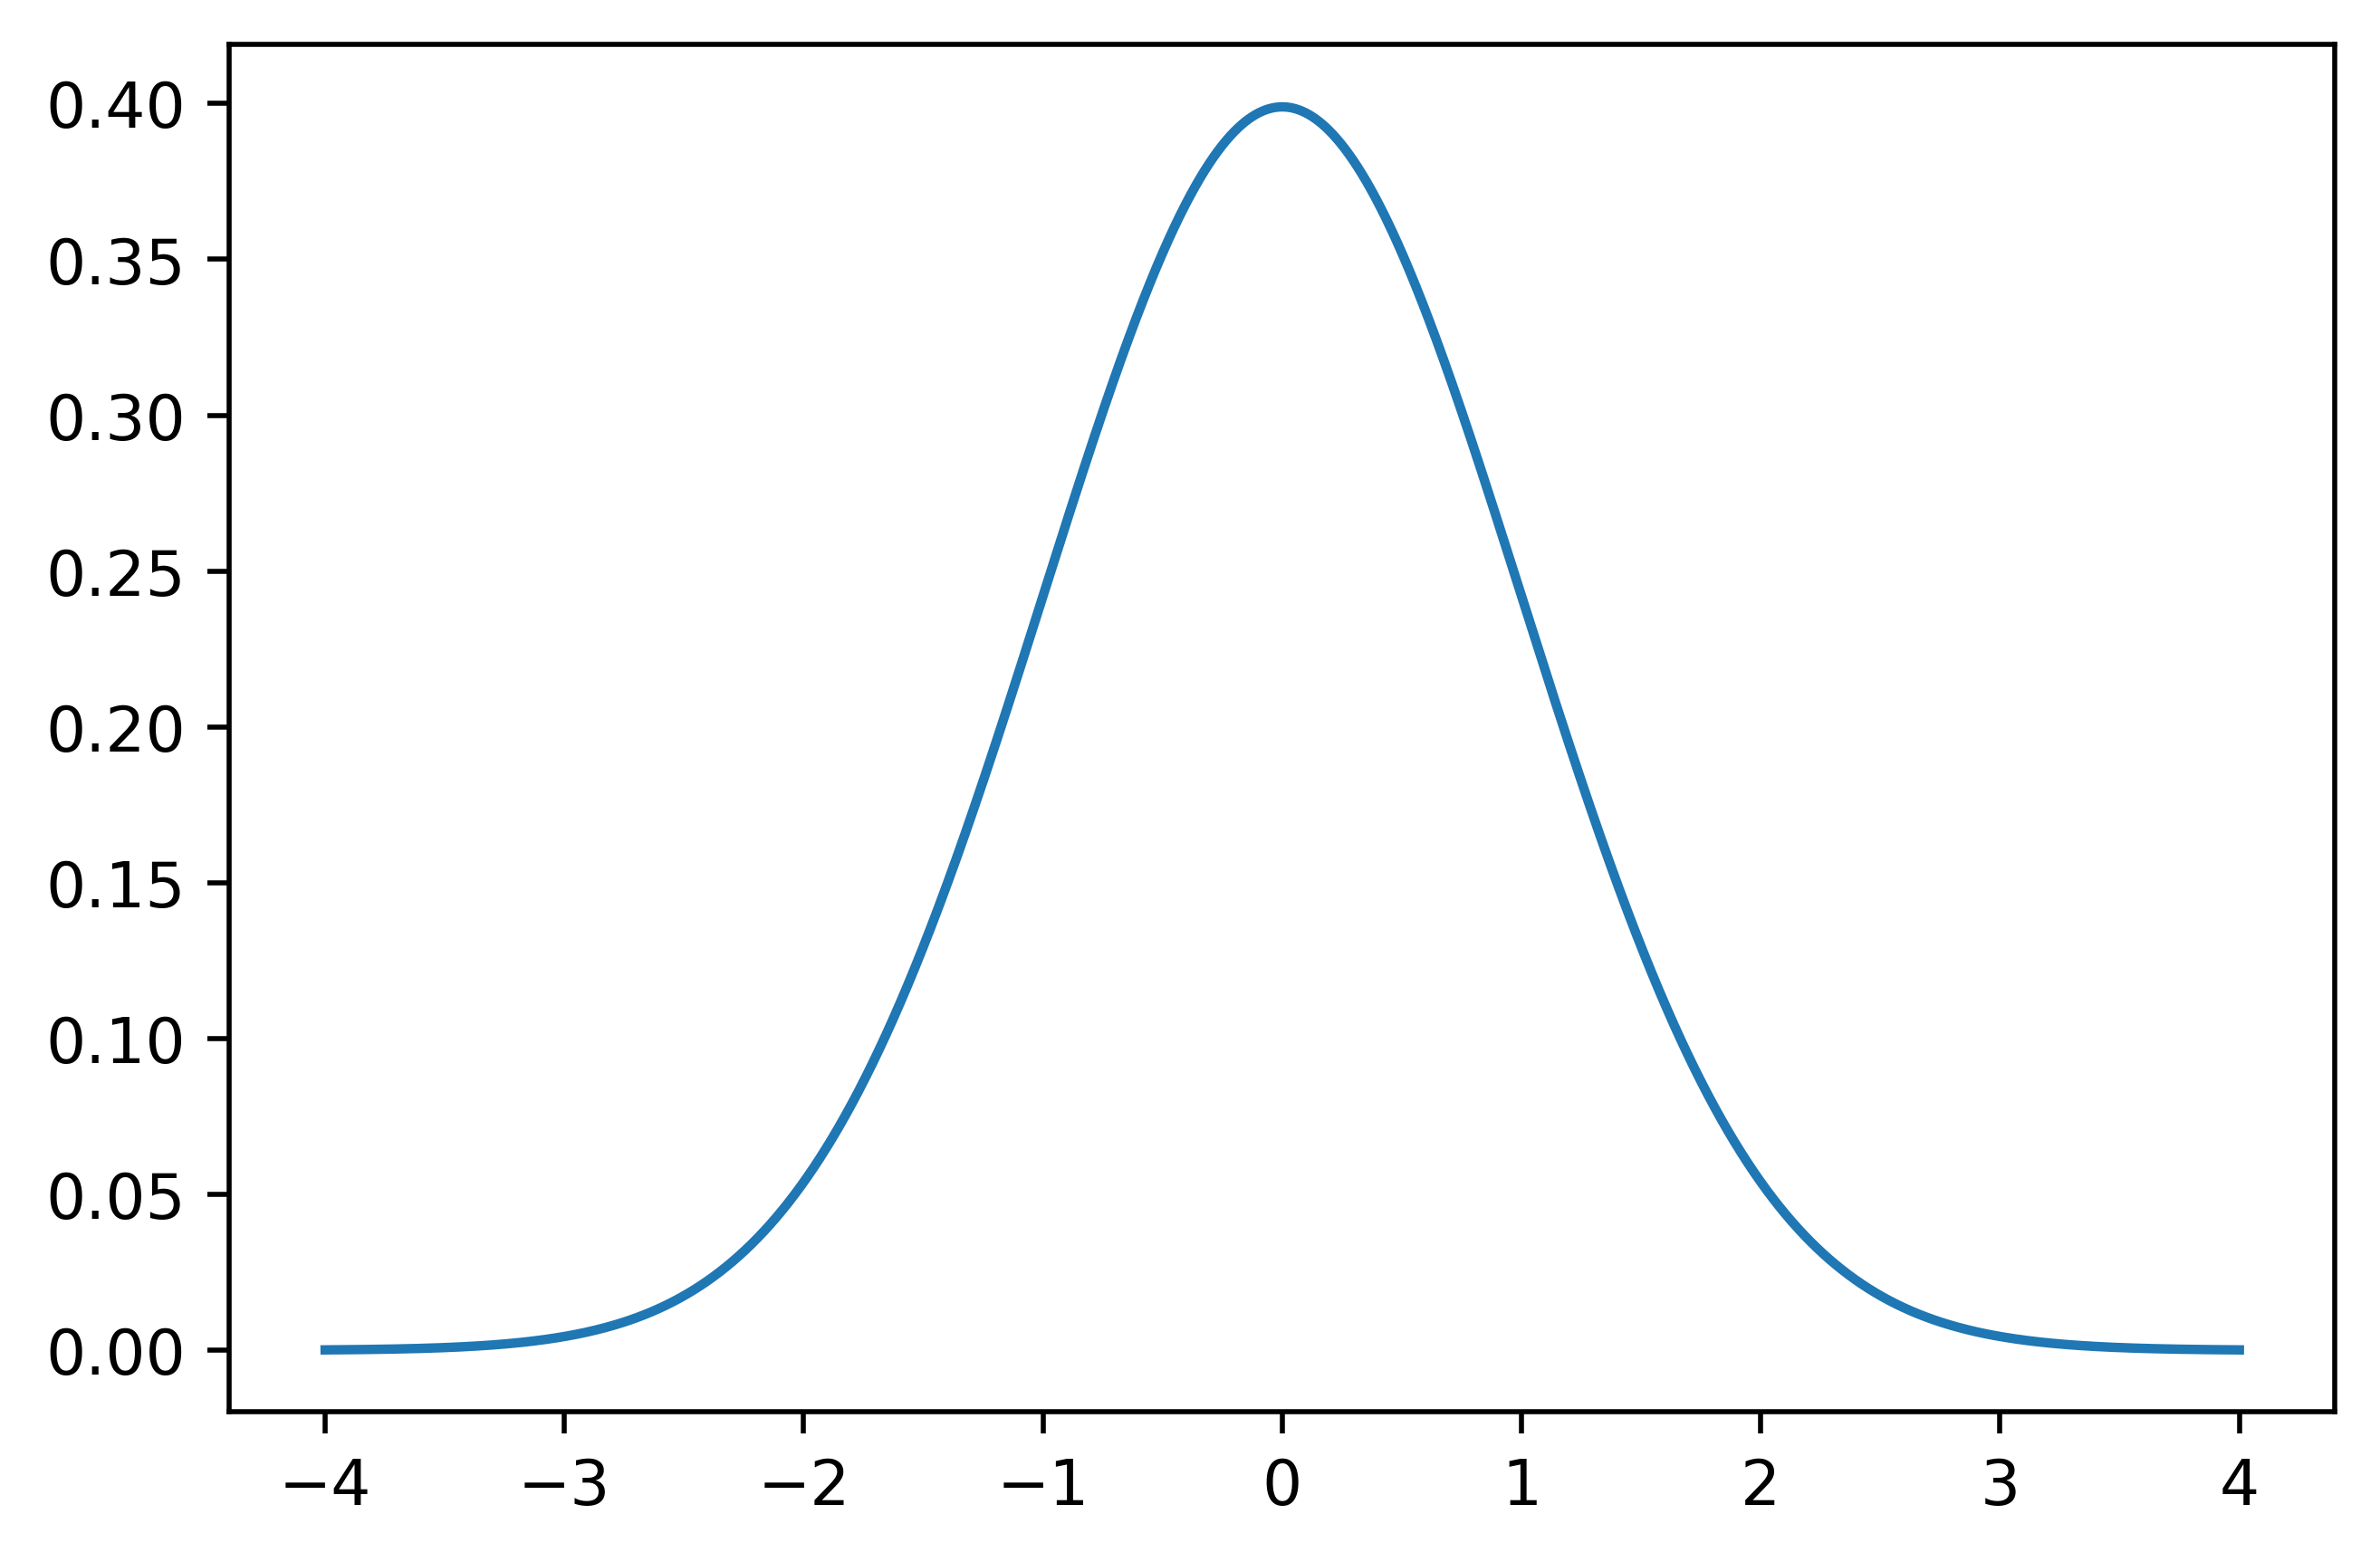
\includegraphics[scale=0.5]{images/gaussian.png}
        \caption{PDF of standard normal distribution}
        \label{normal_pdf}
    \end{figure}
\end{frame}

\begin{frame}{}
 \textbf{Continuous uniform distribution}: Here, we have used U(0, 1). The PMF is given by $$f_X(x) = \begin{cases}1,\; 0 \le x \le 1 \\ 0,\; otherwise\end{cases}$$ 
    The mean is 0.5 and standard deviation is 0.289. Figure \ref{uni_pdf} shows the PDF of the uniform distribution.
\end{frame}
\begin{frame}{}
    \begin{figure}[H]
        \centering
        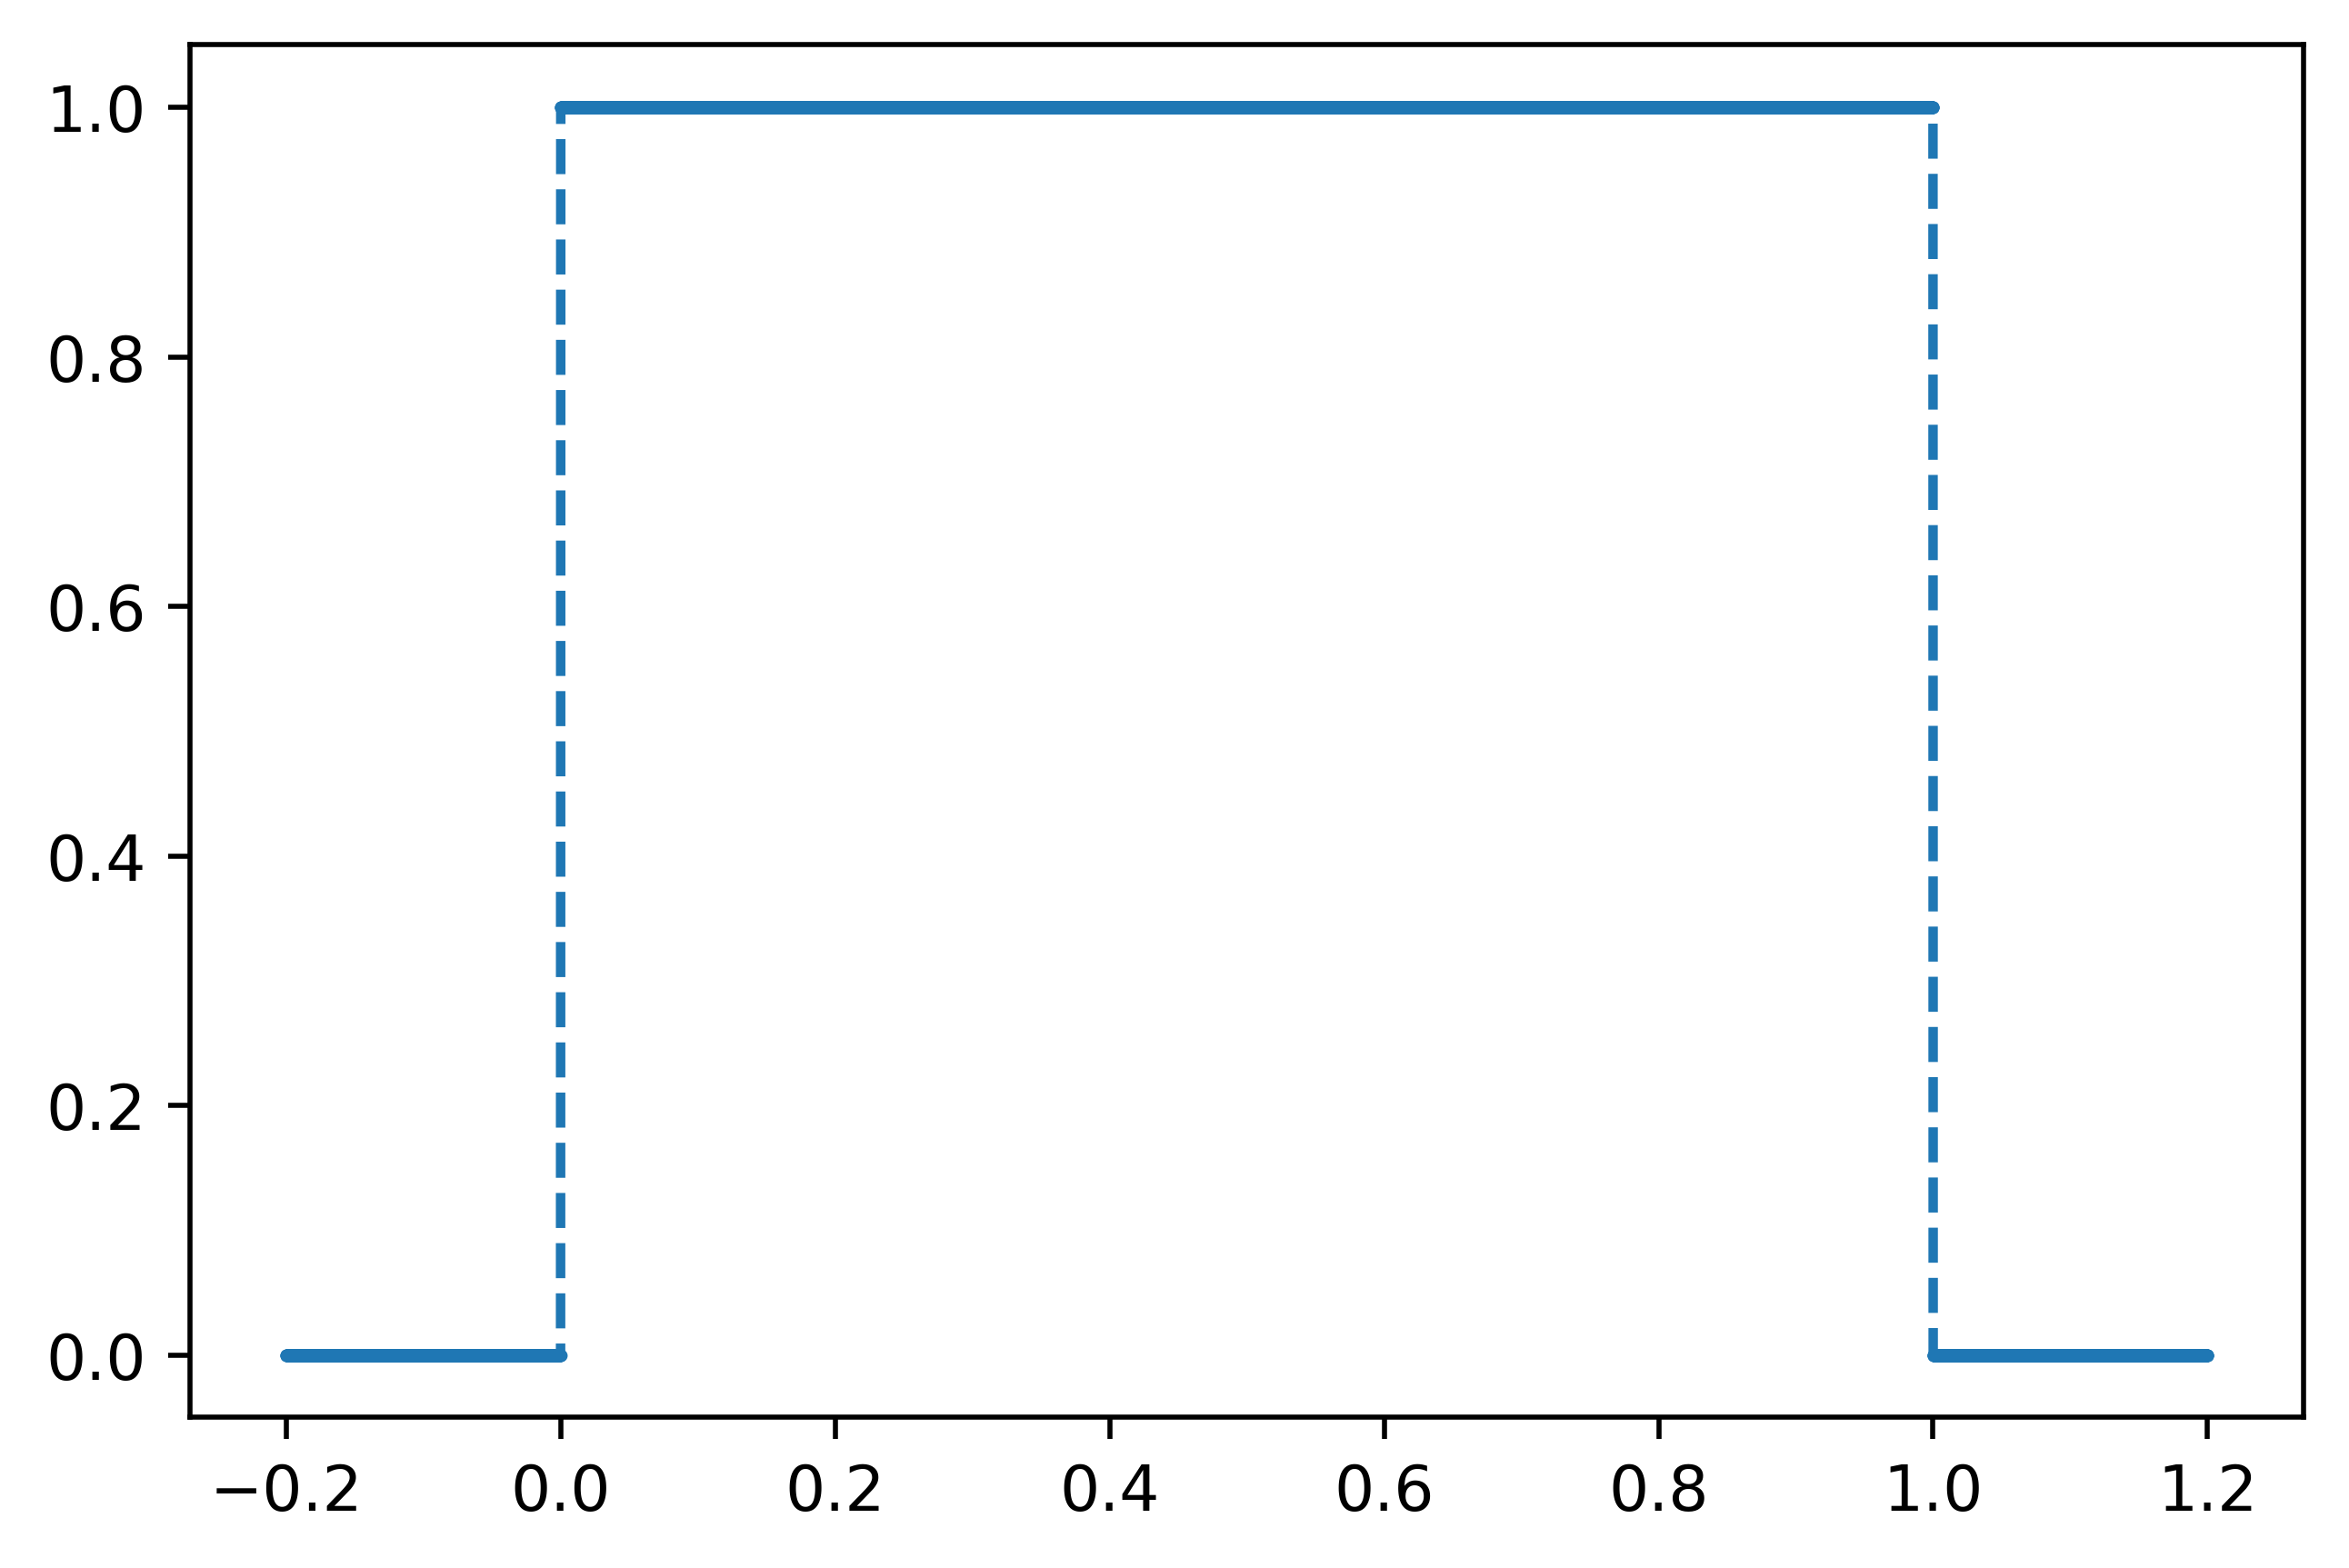
\includegraphics[scale=0.5]{images/uniform.png}
        \caption{PDF of uniform distribution}
        \label{uni_pdf}
    \end{figure}
\end{frame}

\begin{frame}{}
 \textbf{Geometric Distribution}: Unlike the other distributions that we used, this distribution is for a discrete random variable. The PMF is given by
    $$f_X(k) = (1-p)^{k-1}p,\; k=1,2,3,...$$
    In our experiments, we arbitrarily chose to use $p=0.35$. The mean is $\dfrac{1}{p}$ and the standard deviation is $\dfrac{\sqrt{1-p}}{p}$. The PMF is given in figure \ref{geom_pmf}. 
\end{frame}
\begin{frame}{}
    \begin{figure}[H]
        \centering
        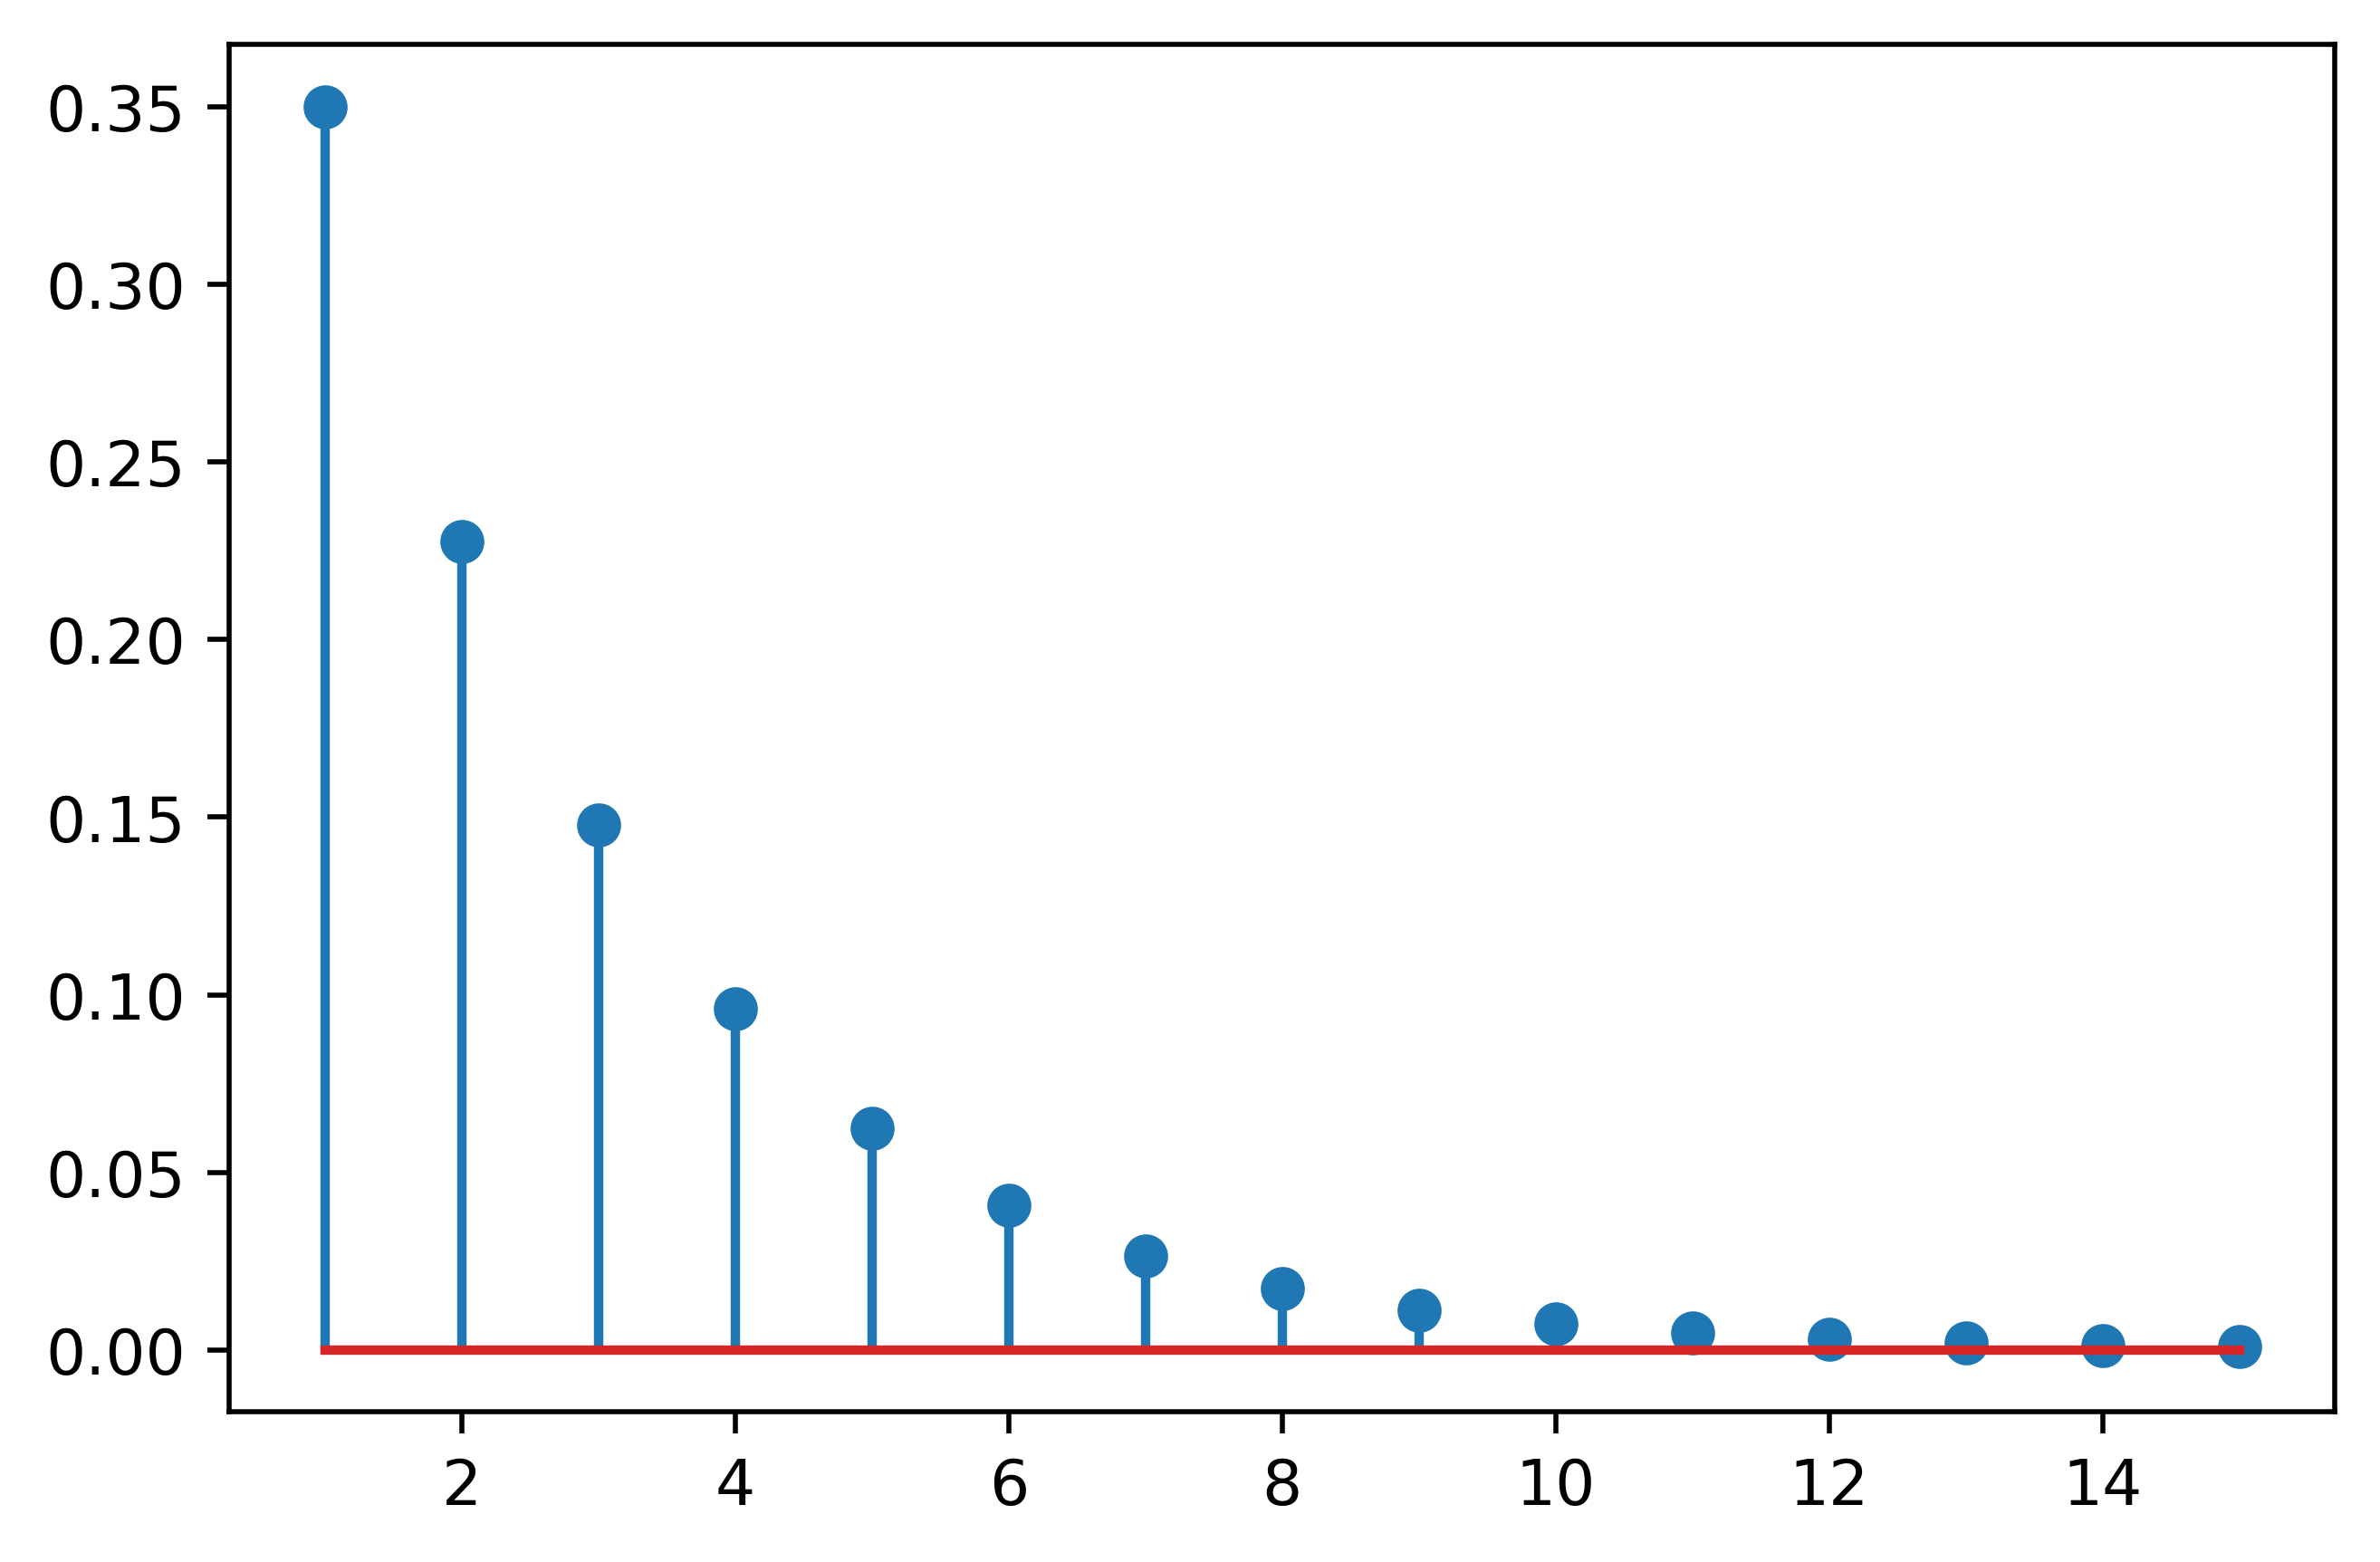
\includegraphics[scale=0.5]{images/geometric.png}
        \caption{PMF of geometric distribution}
        \label{geom_pmf}
    \end{figure}
\end{frame}

\begin{frame}{}
\textbf{Standard cauchy distribution}: The PDF is given by $$f_X(x) = \dfrac{1}{\pi (1+x^2)}$$ Neither the mean nor the standard deviation are finite. Thus CLT should not apply on this distribution. Figure \ref{cauchy_pdf} shows the PDF of standard cauchy distribution.
\end{frame}
\begin{frame}{}
    \begin{figure}[H]
        \centering
        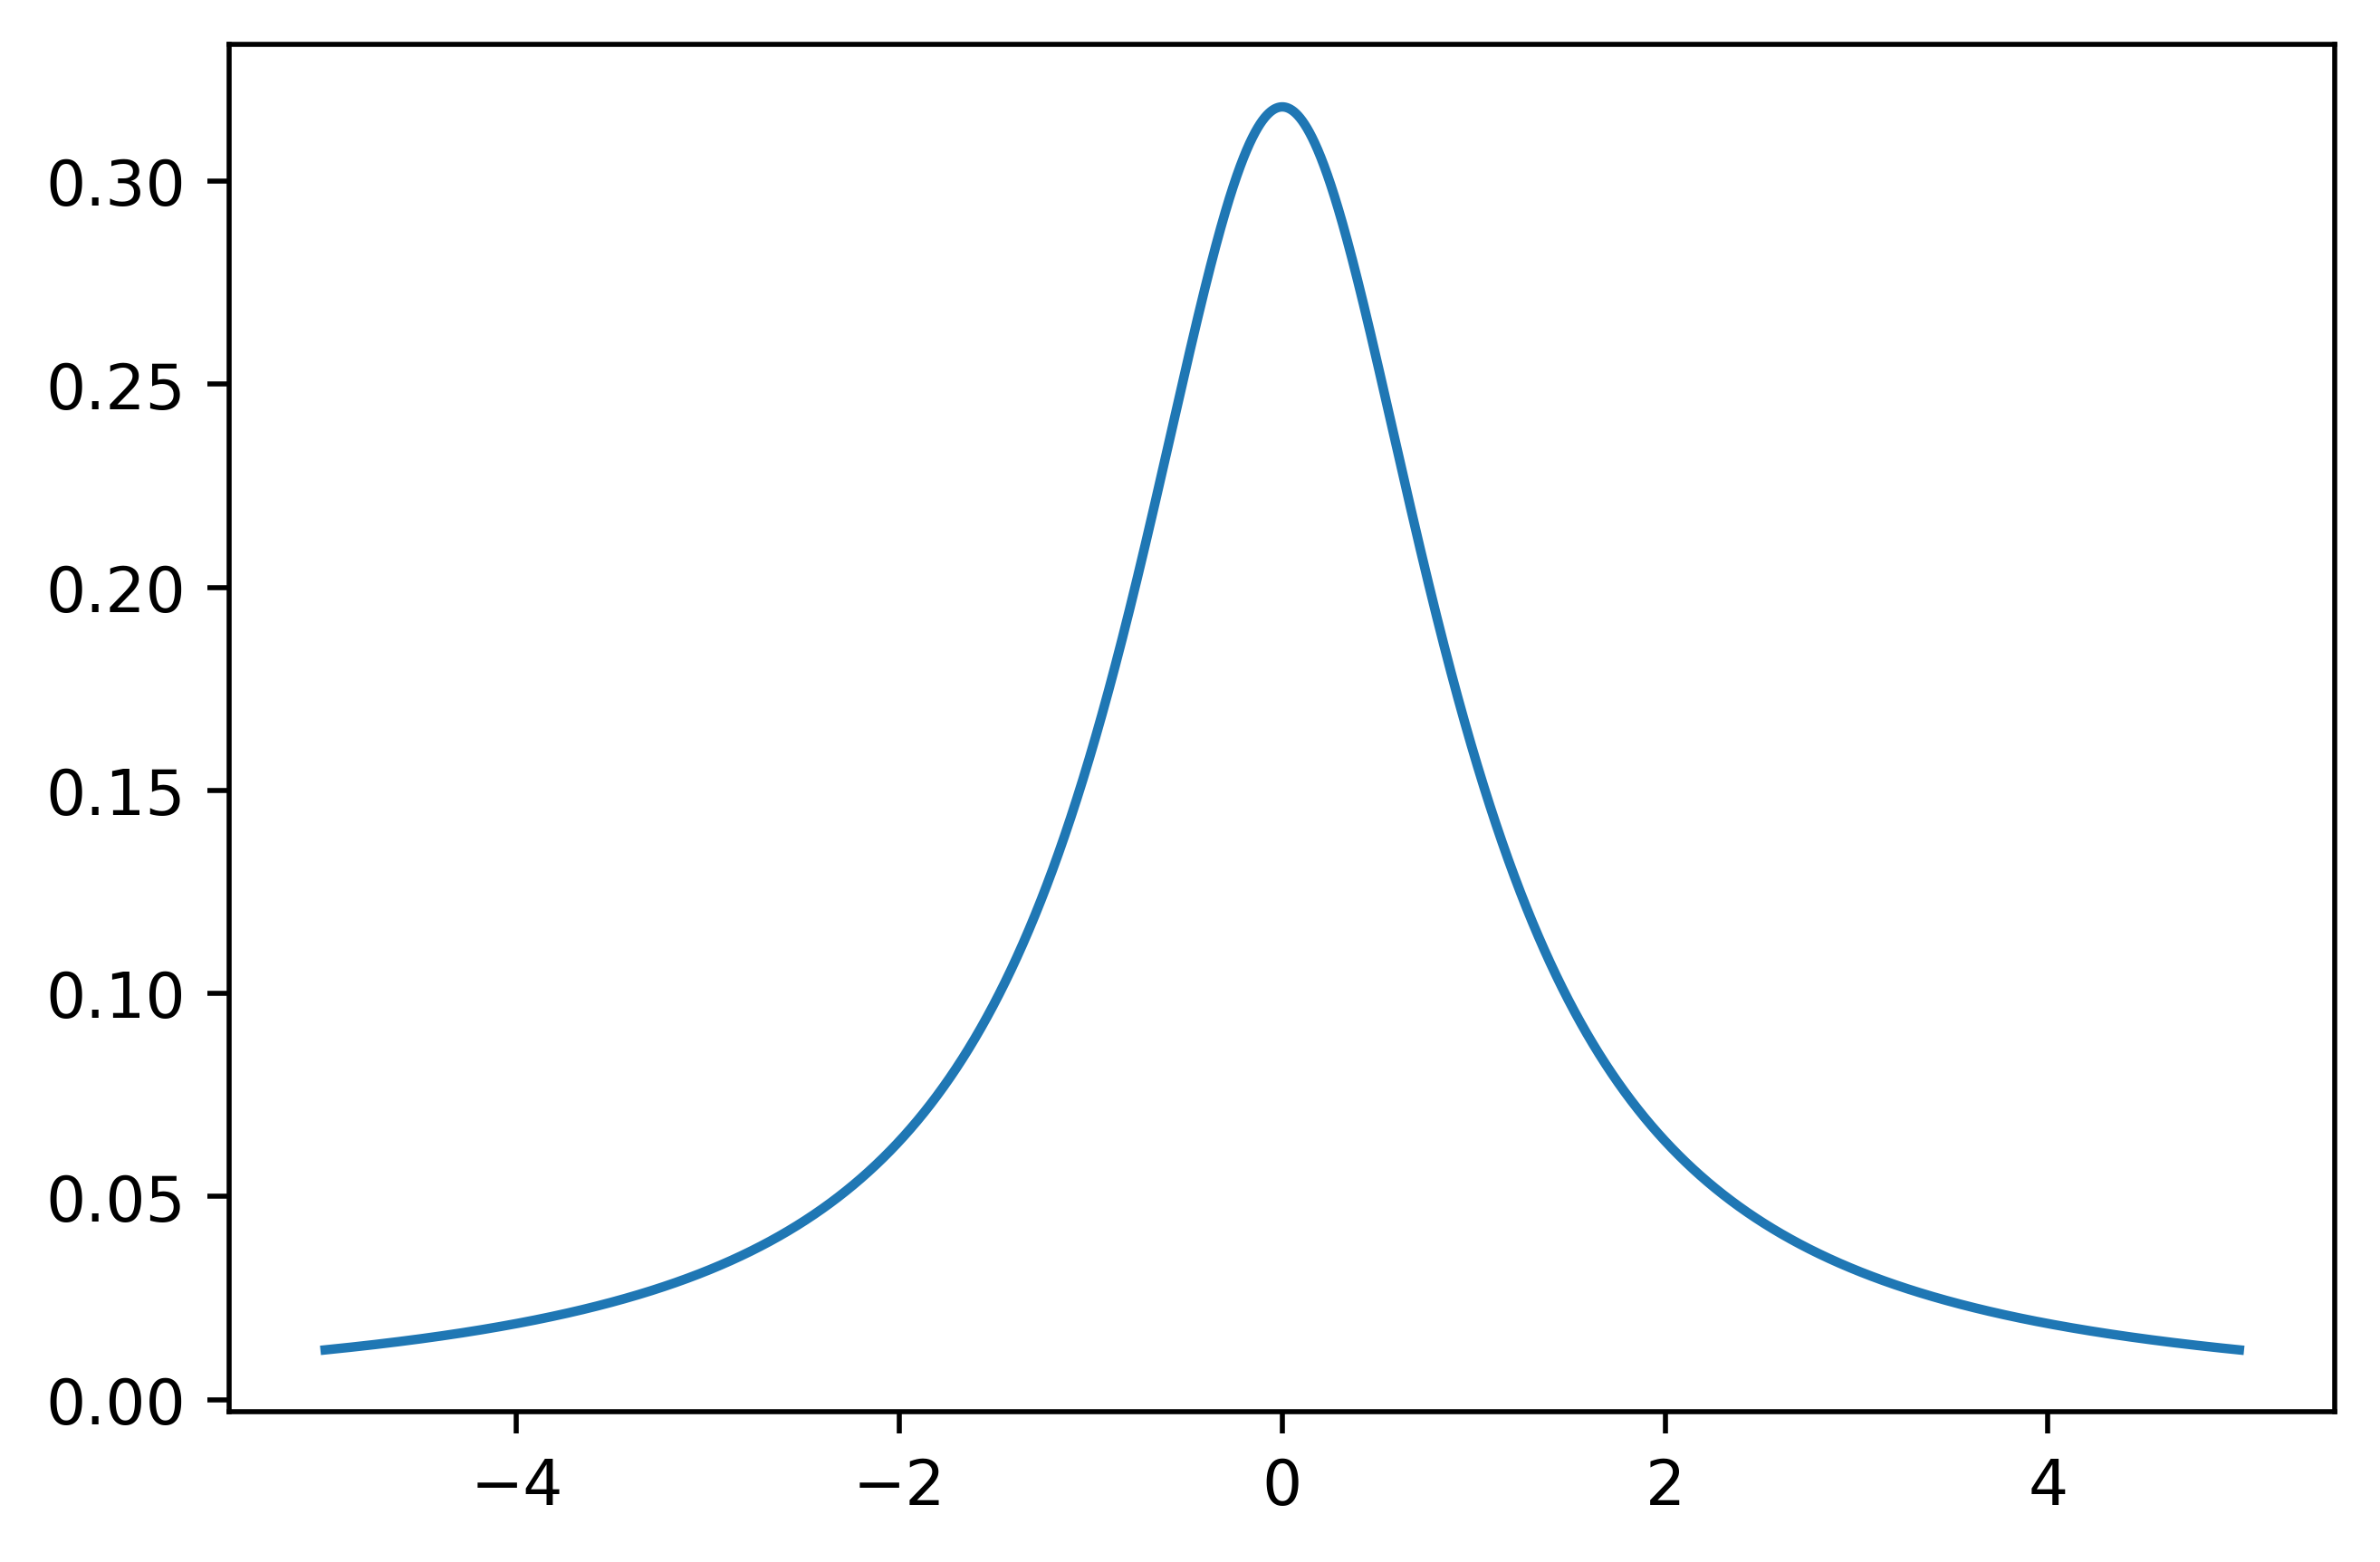
\includegraphics[scale=0.4]{images/cauchy.png}
        \caption{PDF of Cauchy Distribution}
        \label{cauchy_pdf}
    \end{figure}
\end{frame}

% 7th slide
\begin{frame}{Results}
    For Normal distribution and uniform distribution, we found that even for the smallest selected sample size of 10, the sample mean follows Normal distribution as per Shapiro-Wilk test. Thus CLT holds true for these for any sample size greater than or equal to 10. For Geometric distribution, we found that CLT did not hold for sample sizes 10 and 30 as per Shapiro-Wilk test. However, CLT held true for sample sizes 50 and 100. For Cauchy distribution, we found that CLT did not hold for any sample size. 
\end{frame}


% 8th slide
\begin{frame}{Conclusion}
    While using CLT, the empirical approximation is a good one but it may fail. To get better results, one may want to consider using a larger sample size of 50. Also, one may want to verify that the sampling distribution has finite mean and sample variance before applying CLT.
\end{frame}

\begin{frame}{}
\begin{center}
        \Huge{Thank You}
\end{center}
\end{frame}
\end{document}